\documentclass[12pt,a4paper]{article}
\usepackage{graphicx}
\usepackage{biblatex}
\usepackage{parskip}
\usepackage{listings}
\lstset{%
basicstyle=\ttfamily,
breaklines = true,
tabsize=2
}
\graphicspath{ {./Images/} }

\addbibresource{biblography.bib}
\setlength{\parskip}{1em}
\begin{document}
\begin{titlepage}
	\centering
	{\scshape\LARGE ELEC4006 \par}
	\vspace{1cm}
	{\scshape\Large Electronics design project\par}
	\vspace{1.5cm}
	{\huge\bfseries Circuit Simulation Report\par}
	\vspace{2cm}
	{\Large\ Adam\\ Brandon Cann\\ Xin Wang \par}
	\vfill
% Bottom of the page
	{\large \today\par}
\end{titlepage}

\tableofcontents
\pagebreak

\begin{abstract}
This report describes the design and implementation of a program that is capable of performing a transient simulation
by calculating the node voltages at each successive instant in time. This program parses the netlist file
into a graph data structure, performs analysis using conductance matrices and outputs the results in a CSV format.

-- How accurate is it?
\par
-- Comaparison to commercial software?
\end{abstract}
\pagebreak
\section{Overview of the report}
This report is the distillation of multiple research documents relating to different components of the program.
Section 2 gives an abstract view of the design of the program, breaking the program down into 3 modules.
Section 3 provides a summary of the testing methodologies and a comparison to both handwritten results and results of 
established circuit simulator software. 
Section 4 delves into the further work done and some potential ideas to build on.
Section 5, the last section, summarises the report and discusses our overall experiences with the development of this project.

\section{Design}
More in-depth information can be found under research papers of the respective topics.
\par
Object Orientated Programming approach has to be implemented.

\subsection{Parse Netlist}

Format of an circuit description is \cite{spice}:
		$$\tt{<letter><name><node\textit{i}> ... [modelname][parametervalues]}$$
From research, the best type of data structure to express a circuit is a \textbf{Graph Data Structure}.
The graph data structure contains the following member variables:
\begin{itemize}
	\item $\tt{letter}$: Name of component 
	\item $\tt{name}$: Name of node 
	\item $\tt{node1}$: Name of node 1
	\item $\tt{node2}$: Name of node 2
	\item $\tt{compval}$: Value of the component e.g. 5 ohms or 3 volt
\end{itemize}

\par
Aspects to consider regarding input component:
\begin{itemize}
	\item Identifying circuit elements
	\item Support for powers of ten
	\begin{itemize}
		\item When users are entering component values, it is important the program recognises common abbreviations for units
		\item If an abbreviation is not recognised, it is ignored
	\end{itemize} 
\end{itemize}
Aspect to consider regarding storage component:
\begin{itemize}
	\item Proper constructors and deconstructors are implemented
\end{itemize}

\pagebreak
Block diagram depicting the breakdown of Parse Netlist module:
\begin{figure}[h]
    \centering
    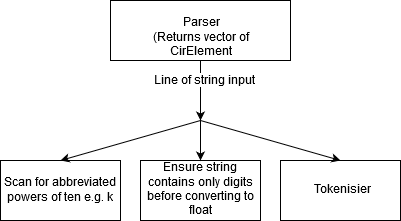
\includegraphics[scale=0.75]{Netlist breakdown}
    \caption{Netlist module breakdown}
    \label{fig:Netlist breakdown}
\end{figure}

Pseudocode implementation: \footnote{Can be expanded to have a textfile containing the library of components supported which can be imported} \footnote{Test scripts and their respective descriptions are found under "Tests Scripts" folder for reference.}
\begin{lstlisting}[language=C++]
	CirElement 
	{
		variables:

			letter: component name
			name: name of node
			node1: node this node is connected to 
			node2: node this node is connected to
			value: float
			initial_val: float

		methods:

			parse(string: input)
			{
				Tokenise
				Put in values into respective variables
				Detect values, pass into custom_pow
				Detect if initial_val is entered:
					Pass into variable otherwise default 0
			}
			custom_pow(string: input)
			{
				Check if there are keywords e.g. k, m, M, G

				If not present, two scenario:
					Unknown letter present: extract digits 
					Convert to float
					Empty string (End of recursion): return 0

				If present:
					Find position where keyword appears
					Take string before keyword and convert
					Multiply/divide the digit by keyword
					Recursion to cover case: 5M7k
			}
			tokeniser(string: input)
			{
				Call regex to tokenise the string 
				Push each token into a vector 
				Return vector
			}
			isdigit(string: input)
			{
				Iterate over string
				Take each character and into 'isdigit' test
				Return boolean
			}
	}
\end{lstlisting}

\par
\pagebreak

\section{Testing}
\subsection{\textit{Data struct}}
The script \textit{Data struct test.sh}, when called, will compile \textit{Data struct.cpp} and passes in input 
text file \textit{Data struct input.txt}. 
\par
\textbf{Pictures}
\par
This test is used to check the format of CirElement data structure functions as envisioned and that the methods associated with
CirElement such as \textit{custom pow} functions correctly.

\pagebreak
\section{Add-on}
\pagebreak
\section{Conclusion}
\pagebreak
\printbibliography[title={References}]
\end{document}